%%%%%%%%%%%%%%%%%%%%%%%%%%%%%%%%%%%%%%%%%
% Short Sectioned Assignment
% LaTeX Template
% Version 1.0 (5/5/12)
%
% This template has been downloaded from:
% http://www.LaTeXTemplates.com
%
% Original author:
% Frits Wenneker (http://www.howtotex.com)
%
% License:
% CC BY-NC-SA 3.0 (http://creativecommons.org/licenses/by-nc-sa/3.0/)
%
%%%%%%%%%%%%%%%%%%%%%%%%%%%%%%%%%%%%%%%%%

%----------------------------------------------------------------------------------------
%	PACKAGES AND OTHER DOCUMENT CONFIGURATIONS
%----------------------------------------------------------------------------------------

\documentclass[paper=a4, fontsize=11pt]{scrartcl} % A4 paper and 11pt font size

\usepackage[T1]{fontenc} % Use 8-bit encoding that has 256 glyphs
\usepackage{fourier} % Use the Adobe Utopia font for the document - comment this line to return to the LaTeX default
\usepackage[english]{babel} % English language/hyphenation
\usepackage{amsmath,amsfonts,amsthm} % Math packages
\usepackage[pdftex]{graphicx}
\graphicspath{{./}}

\usepackage{lipsum} % Used for inserting dummy 'Lorem ipsum' text into the template

\usepackage{sectsty} % Allows customizing section commands
\allsectionsfont{\centering \normalfont\scshape} % Make all sections centered, the default font and small caps

\usepackage{fancyhdr} % Custom headers and footers
\pagestyle{fancyplain} % Makes all pages in the document conform to the custom headers and footers
\fancyhead{} % No page header - if you want one, create it in the same way as the footers below
\fancyfoot[L]{} % Empty left footer
\fancyfoot[C]{} % Empty center footer
\fancyfoot[R]{\thepage} % Page numbering for right footer
\renewcommand{\headrulewidth}{0pt} % Remove header underlines
\renewcommand{\footrulewidth}{0pt} % Remove footer underlines
\setlength{\headheight}{13.6pt} % Customize the height of the header

\numberwithin{equation}{section} % Number equations within sections (i.e. 1.1, 1.2, 2.1, 2.2 instead of 1, 2, 3, 4)
\numberwithin{figure}{section} % Number figures within sections (i.e. 1.1, 1.2, 2.1, 2.2 instead of 1, 2, 3, 4)
\numberwithin{table}{section} % Number tables within sections (i.e. 1.1, 1.2, 2.1, 2.2 instead of 1, 2, 3, 4)

\usepackage{tikz} % Draw graph library

%\setlength\parindent{0pt} % Removes all indentation from paragraphs - comment this line for an assignment with lots of text

%----------------------------------------------------------------------------------------
%	TITLE SECTION
%----------------------------------------------------------------------------------------

\newcommand{\horrule}[1]{\rule{\linewidth}{#1}} % Create horizontal rule command with 1 argument of height

\title{	
\normalfont \normalsize 
\textsc{Network Virtualization and Data Center Networks} \\ [25pt] % Your university, school and/or department name(s)
\horrule{0.5pt} \\[0.4cm] % Thin top horizontal rule
\huge Assignment 2: Cloud computing - software engineer perspective\\ % The assignment title
\horrule{2pt} \\[0.5cm] % Thick bottom horizontal rule
}

\author{Erik Henriksson, Christoph Burkhalter} % Your name

\date{\normalsize\today} % Today's date or a custom date

\begin{document}

\maketitle % Print the title

\section{Proposal}

\subsection{Application}


We will use a simple web-server scenario for the benchmarking and the auto-scaling. There are two types of machines: load-balancers and worker machines. The load-balancers get an IP from a predefined pool of Elastic-IP's such that requests from clients can be sent to them. All load-balancers connect to the overlay network and receive the list of worker machines from the coordinator. Incoming request are sent to a worker machine using a load-balancing technique. In this way load-balancers are connected to all machines in the network, whereas worker machines are only connected to the load-balancers.
The worker machines process the request and contain no further application logic, which means they are not members of the overlay network.
The members of the overlay network (the load-balancers) elect a coordinator and perform a re-electing in case the coordinator dies. We will study the case with exactly two load-balancers, but it is of course easy to scale this up.

\tikzset{
  treenode/.style = {align=center, inner sep=0pt, text centered,
    font=\sffamily},
  load_balancer/.style = {circle, text=white, draw=none,fill=blue},
  node/.style = {circle, text=black, draw=black},
}

\begin{figure}[h!]
\begin{center}
\begin{tikzpicture}[node distance=1cm]
  
  \node [load_balancer] (l1) at (1,2) {L1};
  \node [load_balancer] (l2) at (3,2) {L2};
  \node [node] (n1) at (0,0)  {W1};
  \node [node] (n2) at (2,0) {W2};
  \node [node] (n3) at (4,0)  {W3};

  \foreach \from/\to in {l1/l2,l1/n1,l1/n2,l1/n3,l2/n1,l2/n2,l2/n3}
    \draw (\from) -- (\to);

\end{tikzpicture}
\end{center}

\caption{Network with load balancers (L1,L2) and processing nodes (W1,W2,W3)}
\end{figure}

\subsection{Benchmark}

The benchmark contains latency measurements between machines in the Amazon cloud (cloud to cloud), and a latency test of the application from a client outside the Amazon cloud (client to cloud). The benchmark will be initiated by the coordinator and executed on each machine for the performance benchmark. The latency benchmark is performed on the load-balancers; they test the latency on the network to all running machines in the cloud (other load balancers as well as all the worker machines). These results will be used to optimize load-balancing as well as for the auto scaling.
Additionally,the performance of the system is benchmarked by various workloads (e.g. 1000 request per second from a client). These benchmarks test will be performed with different numbers of worker machines, but a fixed number of two load-balancers.

\subsection{Auto-scaling}

The coordinator in the load balancer network performs the auto-scaling. If the load on the worker machines is too large, the coordinator will start new machines (scale-out). For the scale-out there will be a snapshot with the installed application to improve the start-up time. 
If the workload decreases, the reverse will be done.
In this part we will compare the Amazon load-balancer with our own implementation of a load-balancer, where we detect heavy-loaded machines if the latency increases or from periodically sending ping messages.

\section{Implementation}

erik ...

\section{Problems}

erik ...

\section{Results}

Result description latency (follows...)

\begin{figure*}[h!]
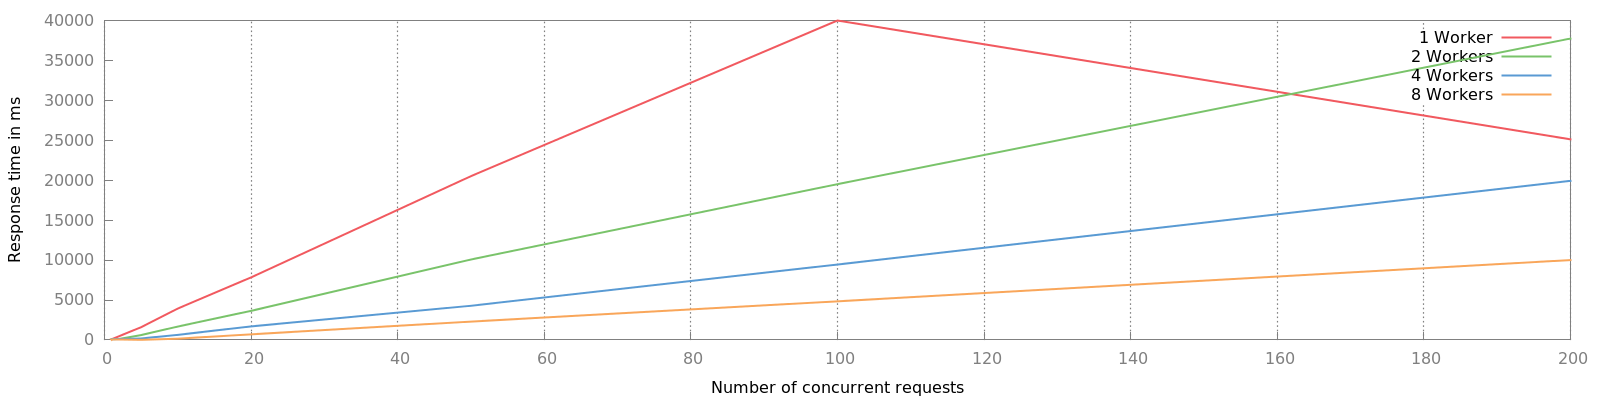
\includegraphics[width=\columnwidth]{../plot/latency_fixed.png}
\end{figure*}

\begin{figure*}[h!]
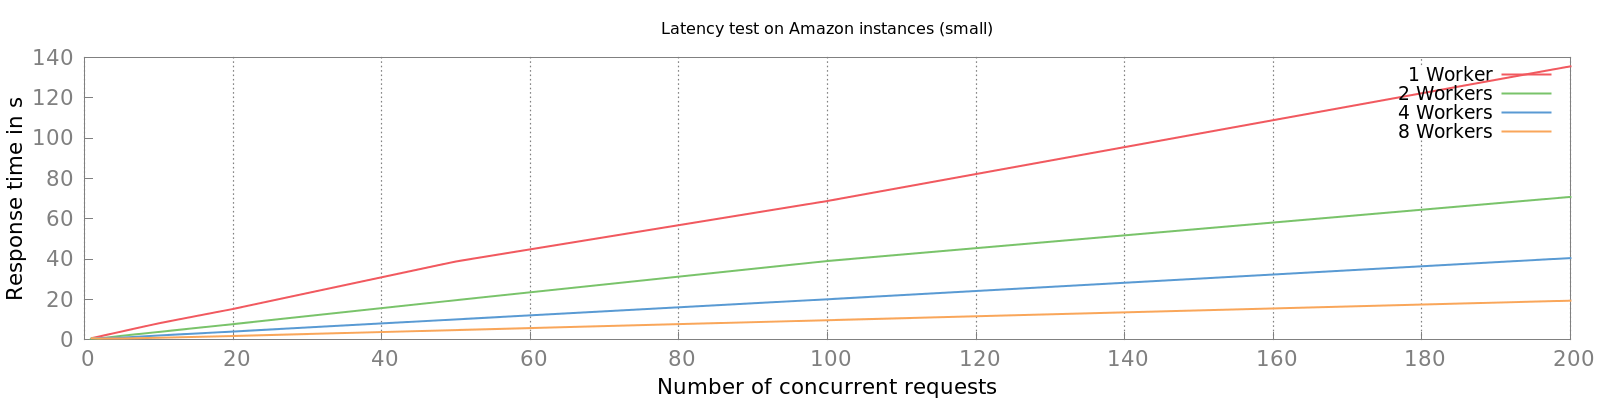
\includegraphics[width=\columnwidth]{../plot/latency_fixed_small.png}
\end{figure*}

Result description workload (follows...)

\begin{figure*}[h!]
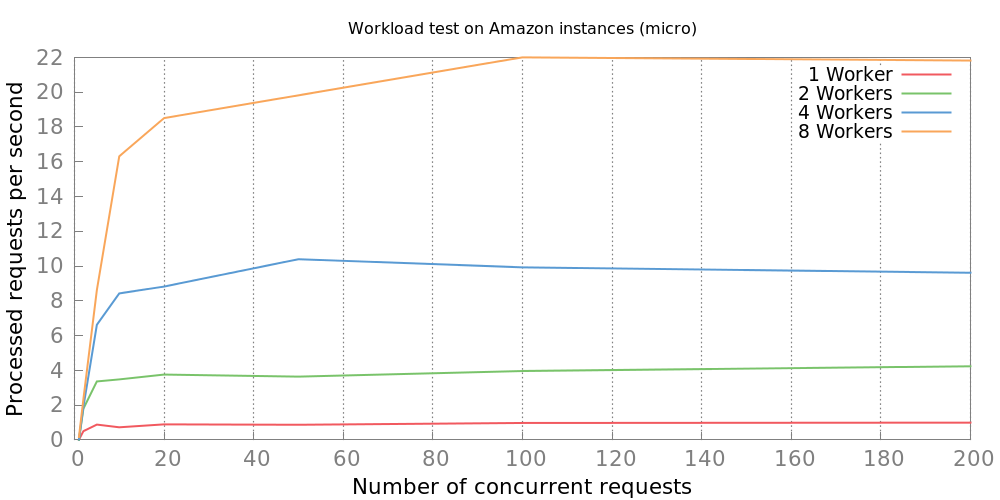
\includegraphics[width=\columnwidth]{../plot/workload.png}
\end{figure*}

\begin{figure*}[h!]
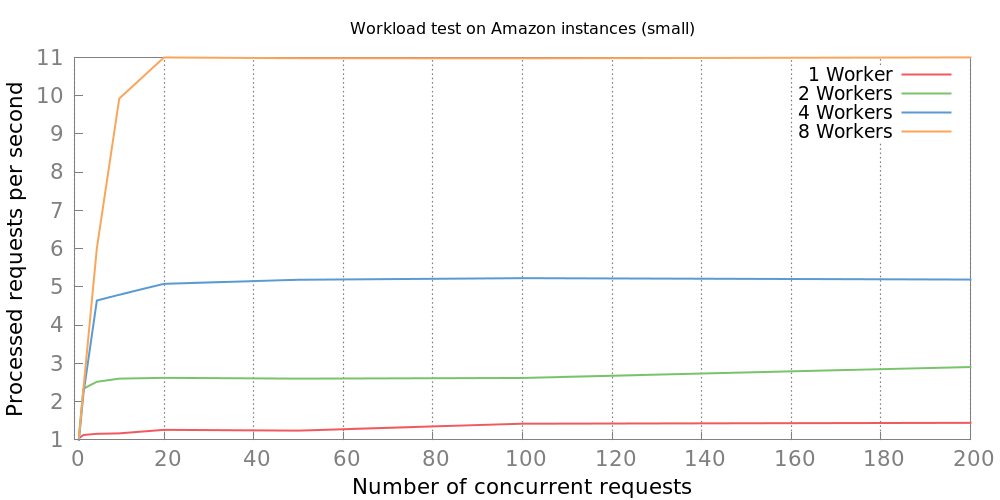
\includegraphics[width=\columnwidth]{../plot/workload_small.png}
\end{figure*}

Result description timeline (follows...)

\begin{figure*}[h!]
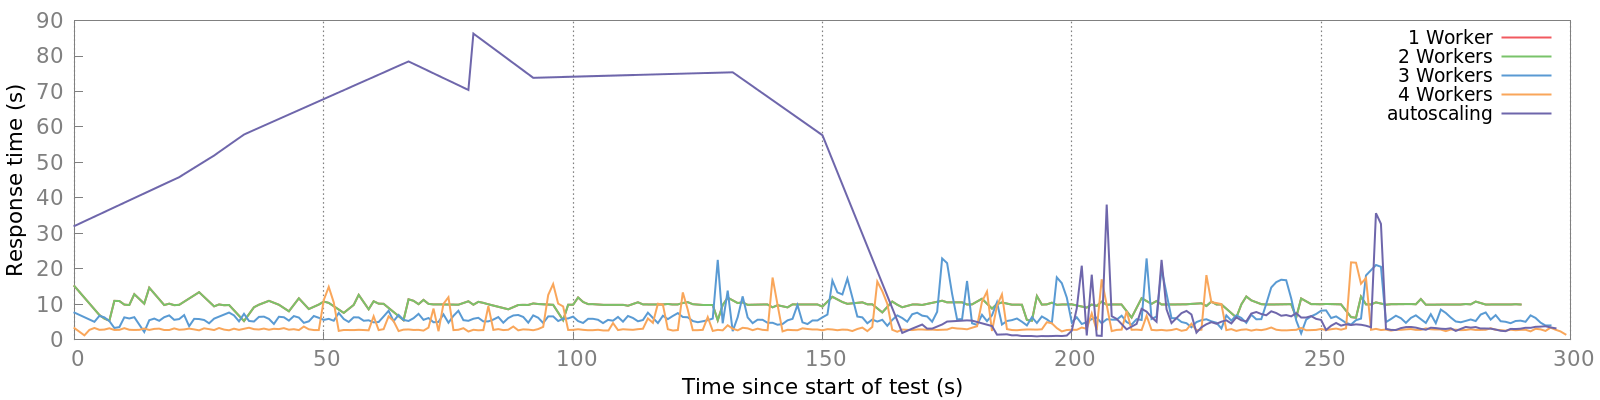
\includegraphics[width=\columnwidth]{../plot/timeline.png}
\end{figure*}

\begin{figure*}[h!]
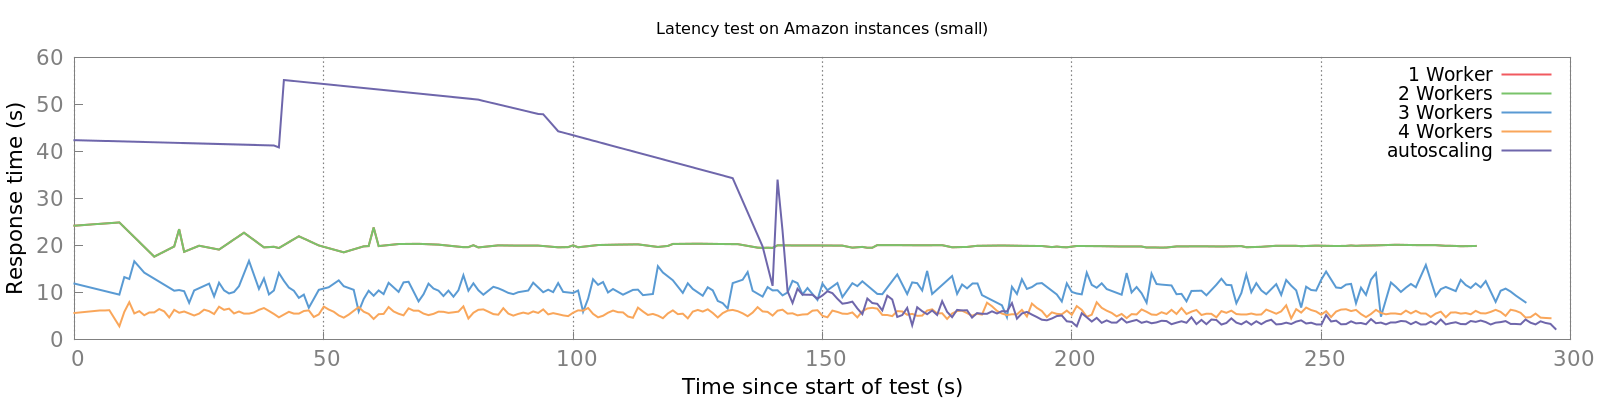
\includegraphics[width=\columnwidth]{../plot/timeline_small.png}
\end{figure*}




\end{document}
